\documentclass[aspectratio=169]{beamer}

\usepackage{beamerthemeinfo}


\title{An example of beamer presentation which is quite very too long. Title}
\subtitle{Subtitles are bloat}
\author{John L. Godlee}

\begin{document}

% \maketitle{background}
\maketitle

\begin{frame}
	\frametitle{First slide example text}
	This is some testy text that explains my point. The text will wrap at some point onto the next line.

	Below is a list with some sample items:

	\begin{itemize}
		\item{item 1}
		\item{Test}
		\item{testy}
	\end{itemize}
\end{frame}

\begin{frame}
	\frametitle{Columns are good}
	\begin{columns}
		\column{0.45\textwidth}

		This is some text in a column that spans just under half the page width. On the right hand side is an image.

		\column{0.55\textwidth}
		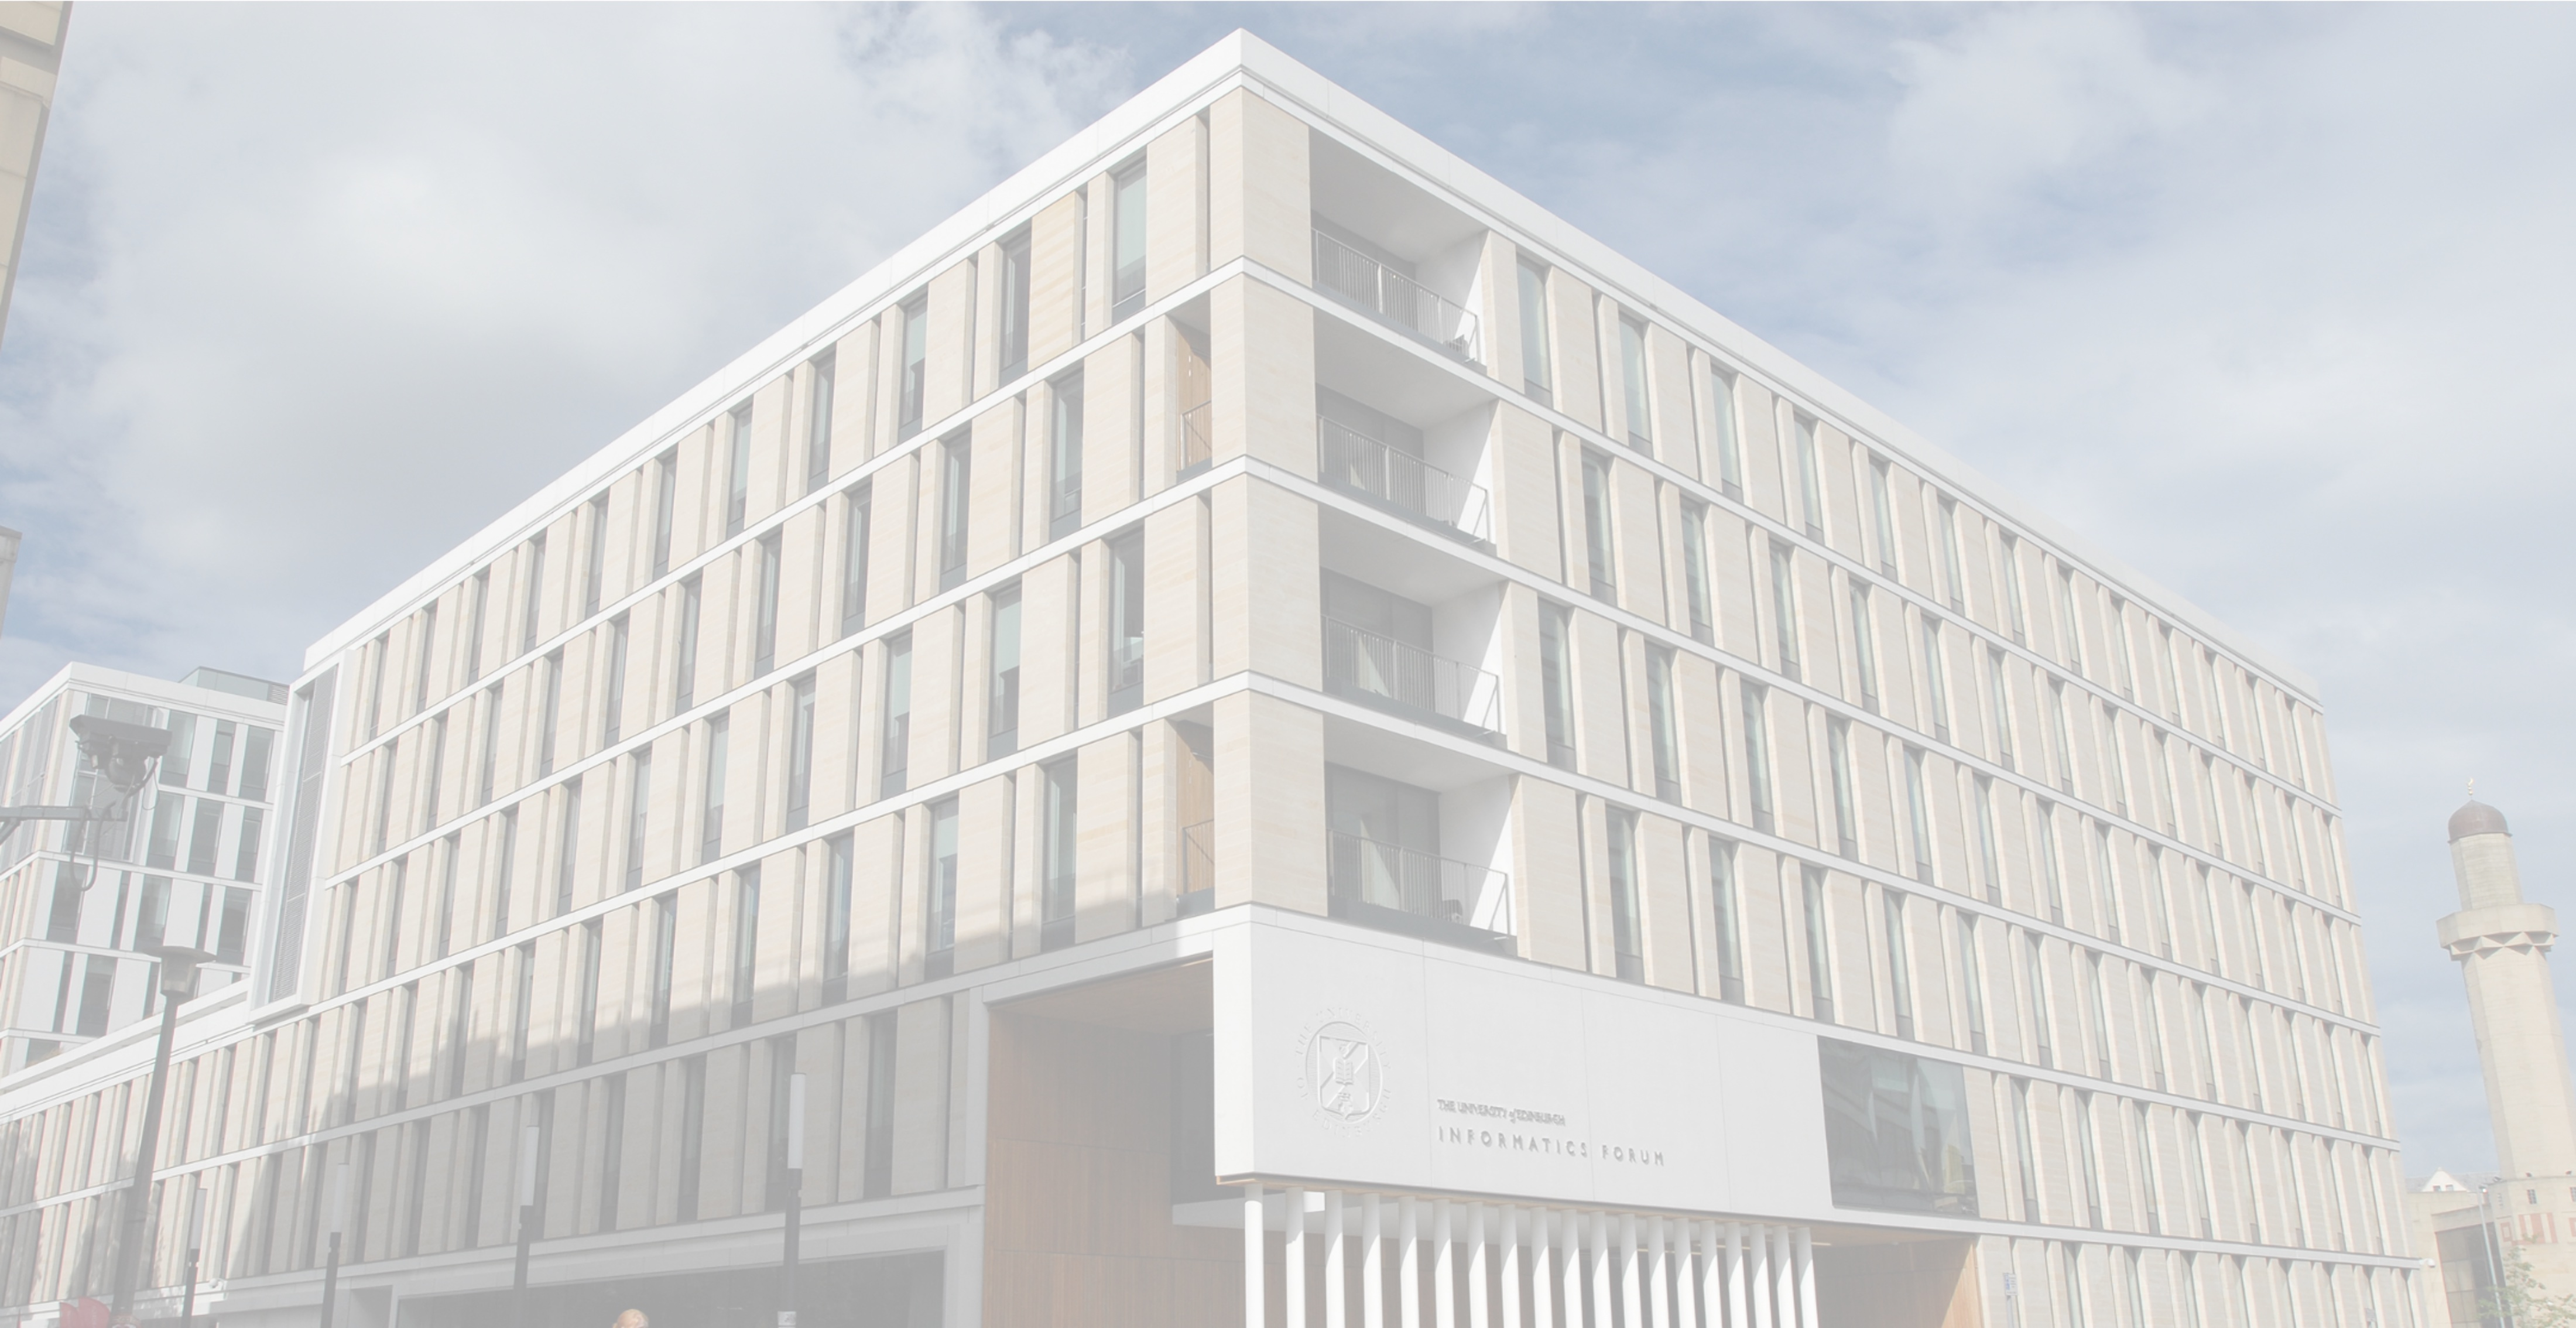
\includegraphics[width=\textwidth]{background}
	\end{columns}
\end{frame}

\begin{frame}{TITLE}
	\begin{block}{Block contain stuff}
		The body of the block. that is pretty long actually look it goes over two lines by now hopefully. The block is used for definitions and whatnot
	\end{block}
	\begin{alertblock}{Alert block}
		OHHH SHIITTT, this must be really important.
	\end{alertblock}
	\begin{exampleblock}{Example block}
		An example of something awesome.
	\end{exampleblock}
\end{frame}

\end{document}
